\section{Clase 5 de junio}

Si \(C_p = 87\),
\(G = 10\),
\(I = 6\),
\(Ex = 4\),
\(Im = 7\).

Notar que balanza comercial es negativa.
Si operamos, obtenemos:

\begin{equation*}
    PIB = 97 + 10 + 6 + 4 - 7 = \boxed{110}
\end{equation*}

El PIB es un indicador más que hay que tener en cuenta
para evaluar la situación de un país.

\subsection{PIB per cápita}

El PIB per cápita se obtiene dividiendo
PIB total por la cantidad de habitantes en un año.

\subsection{Errores/defectos en el PIB}

El PIB se considera como una herramienta para de alguna manera indicar
"cierta riqueza de un país", o como medida del bienestar generalizado.
Pero estas cifras deben ser observadas con cuidado,
ya que no tienen en cuenta ciertas situaciones como algunas de las siguientes:
\begin{enumerate}
    \item No considera ciertas externalidades negativas,
          como por ejemplo la contaminación ambiental.
    \item No tiene en cuenta la distribución del ingreso,
          es decir,
          el PIB per cápita no es un indicador de distribución por persona,
          sino más bien un indicador del tipo promedio.
    \item El PIB no tiene en cuenta las transacciones de trabajos como
          voluntariado y amas de casa.
    \item Hay actividades negativas que tienden a aumentar el valor del PIB,
          como por ejemplo los honorarios de abogados que defienden criminales,
          o los sueldos de guardacárceles.
    \item No tiene en cuenta la deuda externa.
    \item No tiene en cuenta ciertos \textit{ratios} como la inflación.
    \item No tiene en cuenta costos sociales como el desempleo,
          el empleo infantil, la asistencia social que hacen los estados.
    \item No tiene en cuenta la calidad de los artículos fabricados y
          la piratería o falsificación.
    \item No mide la eficacia de la asignación de los recursos.
    \item No mide el despilfarro del dinero por ineficiencias.
    \item No mide impactos negativos; una obra que tiene malas
          consecuencias igualmente se cuenta como positiva.
\end{enumerate}


\vspace{.5cm}
\begin{table}[H]
    \centering
    \caption{\\Ranking PIB per cápita global}
    \begin{tabular}{rlllll}
        \hline
          & 1870         & 1900         & 1929         & 1950         & 2004         \\
        1 & Australia    & Reino Unido  & EE. UU.      & Qatar        & Luxemburgo   \\
        2 & R. Unido     & N. Zelanda   & Suiza        & Kwait        & Noruega      \\
        3 & N. Zelanda   & EE. UU.      & Holanda      & Em. Árabes   & Suiza        \\
          & \(\cdots\)   & \(\cdots\)   & \(\cdots\)   & \(\cdots\)   & \(\cdots\)   \\
          & 18 Argentina & 13 Argentina & 11 Argentina & 17 Argentina & 91 Argentina \\
        \hline
    \end{tabular}
\end{table}
\vspace{.5cm}

\subsection{Fluir del ingreso a través del sistema económico}

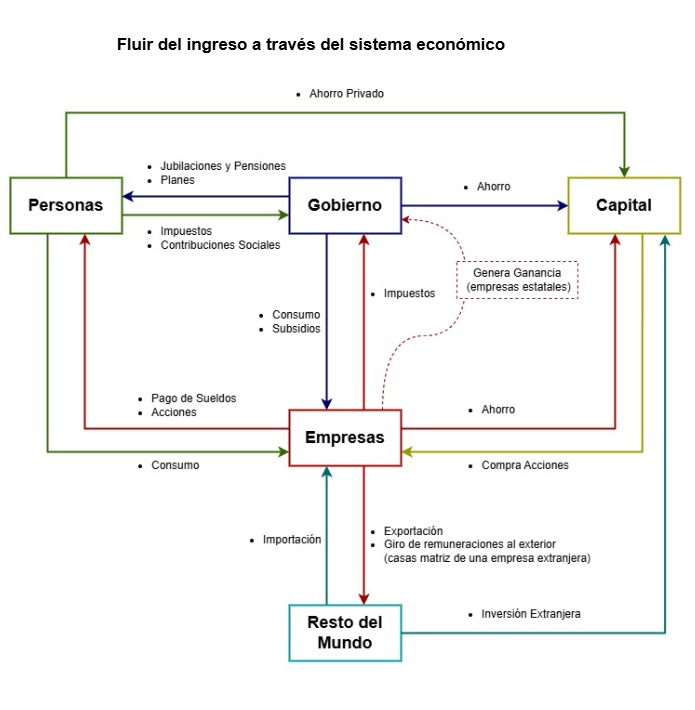
\includegraphics[width=\textwidth]{img/flujo-del-ingreso.jpeg}